\subsubsection{UC4 - Selezione dizionario dati}\label{UC4}

\begin{figure}[H]
  \centering
  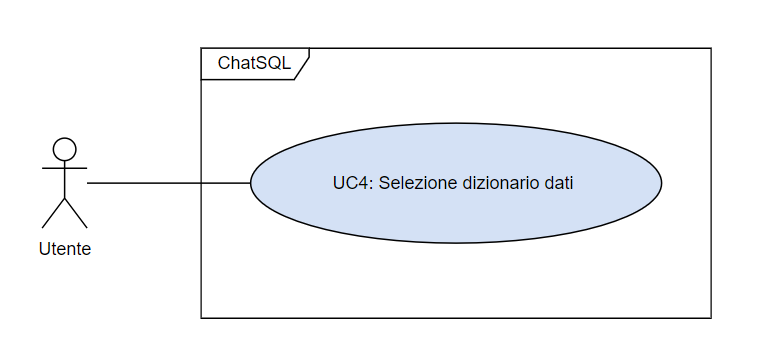
\includegraphics[width=0.90\textwidth]{assets/uc4.png}
  \caption{UC4}
\end{figure}

\paragraph*{Descrizione}
L'Utente seleziona un \glossario{dizionario dati} da utilizzare nel sistema.

\paragraph*{Attori principali}
Utente

\paragraph*{Precondizioni}
\begin{itemize}
  \item L'applicazione è stata avviata con successo;
  \item Nel sistema è stato caricato almeno un \glossario{dizionario dati} (\hyperref[UC13]{UC13}).
\end{itemize}

\paragraph*{Postcondizioni}
\begin{itemize}
  \item Il \glossario{dizionario dati} è stato selezionato in modo corretto;
  \item Il dizionario dati è ora attivo nel sistema.
\end{itemize}

\paragraph*{Trigger}
L'Utente vuole selezionare un \glossario{dizionario dati} da utilizzare nell'applicazione.

\paragraph*{Scenario principale}
\begin{enumerate}
  \item L'Utente sceglie un \glossario{dizionario dati} tra quelli disponibili.
\end{enumerate}